% Conference-length manuscript. Build and export through the Make targets.
% The longer version 4 report is retained separately in report-v4.tex.
\documentclass[10pt,letterpaper,twocolumn]{article}
\usepackage[T1]{fontenc}
\usepackage{lmodern}
\usepackage[margin=1in]{geometry}
\usepackage{microtype}
\usepackage{amsmath,amssymb,amsthm}
\usepackage{booktabs,array}
\usepackage{flafter}
\usepackage{placeins}
\usepackage{xcolor}
\usepackage{graphicx}
\usepackage{tikz}
\usetikzlibrary{arrows.meta,positioning}
\usepackage{pgfplots}
\pgfplotsset{compat=1.18}
\usepackage{listings}
\usepackage{enumitem}
\usepackage{fancyhdr}
\usepackage{url}
\usepackage[colorlinks=true,linkcolor=blue!45!black,citecolor=blue!45!black,urlcolor=blue!45!black]{hyperref}
\definecolor{ink}{HTML}{214E70}
\definecolor{accent}{HTML}{B85C38}
\definecolor{pale}{HTML}{F3F5F7}
\hypersetup{pdftitle={Resumable FFT Scheduling for Real-Time Spectral Analysis},pdfauthor={Christian Kauten},pdfsubject={Technical report on cooperative FFT scheduling, latency, and reproducible evaluation},pdfkeywords={FFT, STFT, cooperative scheduling, real-time audio, spectrum analysis, VCV Rack}}
\pagestyle{fancy}
\fancyhf{}
\fancyhead[L]{\small\textsc{Resumable FFT Scheduling}}
\fancyhead[R]{\small Technical report}
\fancyfoot[C]{\thepage}
\setlength{\headheight}{14pt}
\setlength{\emergencystretch}{2em}
\setlist{nosep}
\newtheorem{proposition}{Proposition}
\newcommand{\code}[1]{\texttt{#1}}
\newcommand{\ceil}[1]{\left\lceil #1\right\rceil}
\newcommand{\floor}[1]{\left\lfloor #1\right\rfloor}
\newcommand{\repo}{\url{https://github.com/Kautenja/ArhythmeticUnits-Fourier}}
\lstset{basicstyle=\ttfamily\footnotesize,keywordstyle=\color{ink}\bfseries,commentstyle=\color{black!55},stringstyle=\color{accent},backgroundcolor=\color{pale},frame=single,rulecolor=\color{black!15},breaklines=true,columns=fullflexible,keepspaces=true,showstringspaces=false,tabsize=4,captionpos=b,xleftmargin=0.5em,xrightmargin=0.5em}

% Generated by tools/study_paper.py; do not edit.
\newcommand{\StudyBatchCost}{68.3}
\newcommand{\StudyBatchPeak}{52.2}
\newcommand{\StudyCoreCost}{80.3}
\newcommand{\StudyCorePeak}{6.67}
\newcommand{\StudyEmptyCpuCores}{3.01}
\newcommand{\StudyHorizonFullCost}{589}
\newcommand{\StudyHorizonFullPeak}{68.6}
\newcommand{\StudyHorizonHalfCost}{594}
\newcommand{\StudyHorizonHalfPeak}{95.4}
\newcommand{\StudyHorizonQuarterCost}{568}
\newcommand{\StudyHorizonQuarterPeak}{121}
\newcommand{\StudyHostBatchBudgetPercent}{66.7}
\newcommand{\StudyHostBatchCost}{1730}
\newcommand{\StudyHostBatchMisses}{20}
\newcommand{\StudyHostBatchPeak}{890}
\newcommand{\StudyHostCoreBudgetPercent}{15.1}
\newcommand{\StudyHostCoreCost}{2300}
\newcommand{\StudyHostCoreMisses}{18}
\newcommand{\StudyHostCorePeak}{201}
\newcommand{\StudyHostFftwBatchBudgetPercent}{64.6}
\newcommand{\StudyHostFftwBatchCost}{1650}
\newcommand{\StudyHostFftwBatchMisses}{419}
\newcommand{\StudyHostFftwBatchPeak}{861}
\newcommand{\StudyHostHybridBudgetPercent}{31.7}
\newcommand{\StudyHostHybridCost}{2040}
\newcommand{\StudyHostHybridMisses}{38}
\newcommand{\StudyHostHybridPeak}{423}
\newcommand{\StudyHostManyBatchBudgetPercent}{19.6}
\newcommand{\StudyHostManyBatchCost}{1760}
\newcommand{\StudyHostManyBatchMisses}{0}
\newcommand{\StudyHostManyBatchPeak}{261}
\newcommand{\StudyHostManyCoreBudgetPercent}{10.8}
\newcommand{\StudyHostManyCoreCost}{1740}
\newcommand{\StudyHostManyCoreMisses}{19}
\newcommand{\StudyHostManyCorePeak}{144}
\newcommand{\StudyHostStaggerBatchBudgetPercent}{12.8}
\newcommand{\StudyHostStaggerBatchCost}{1940}
\newcommand{\StudyHostStaggerBatchMisses}{36}
\newcommand{\StudyHostStaggerBatchPeak}{171}
\newcommand{\StudyModuleBothBudgetPercent}{91.7}
\newcommand{\StudyModuleBothComputeMisses}{196}
\newcommand{\StudyModuleBothMisses}{583}
\newcommand{\StudyModuleBothPeak}{1220}
\newcommand{\StudyModuleDefaultBudgetPercent}{3.12}
\newcommand{\StudyModuleDefaultComputeMisses}{0}
\newcommand{\StudyModuleDefaultMisses}{21}
\newcommand{\StudyModuleDefaultPeak}{41.6}
\newcommand{\StudyModuleExtremeBudgetPercent}{74.7}
\newcommand{\StudyModuleExtremeComputeMisses}{10}
\newcommand{\StudyModuleExtremeMisses}{256}
\newcommand{\StudyModuleExtremePeak}{997}
\newcommand{\StudyPffftBatchCost}{41.3}
\newcommand{\StudyPffftBatchPeak}{13.7}
\newcommand{\StudyPffftHybridCost}{49.8}
\newcommand{\StudyPffftHybridPeak}{8.15}
\newcommand{\StudyPlacementComparisons}{24}
\newcommand{\StudyPlacementCostRatio}{1.18}
\newcommand{\StudyPlacementRatio}{7.82}
\newcommand{\StudyPlacementSigns}{24}
\newcommand{\StudySimdExtremeCost}{1080}
\newcommand{\StudySimdExtremePeak}{93.6}
\newcommand{\StudyVdspBatchCost}{43.6}
\newcommand{\StudyVdspBatchPeak}{17.1}
\newcommand{\StudyVdspHybridCost}{59.4}
\newcommand{\StudyVdspHybridPeak}{8.92}

\title{\textbf{Scheduling FFT-Based Spectral Analysis\\in the Audio Processing Loop}}
\author{Christian Kauten\\Arhythmetic Units\\\small\href{mailto:arhythmetic.units@gmail.com}{arhythmetic.units@gmail.com}}
\date{October 1, 2026\quad /\quad Preprint, manuscript version 5}

\begin{document}
\twocolumn[\maketitle
\begin{abstract}
\noindent
An FFT-based spectrum analyzer can be inexpensive on average yet concentrate
most of its work in one audio-processing call. This paper describes how to
spread that work across successive sample calls without a separate analysis
thread. A resumable radix-2 FFT preserves its traversal state between calls;
windowing, spectrum reconstruction, smoothing, and output preparation are
scheduled alongside it. Each frame completes over one chosen update interval,
with a bounded operation count per call and an explicit delay before the
spectrum becomes available. We implement the method in two VCV Rack
visualizers and evaluate it using matched batch controls and optimized native
FFT libraries. In a scalar 4096-point comparison, distributing the same
implementation reduces the typical peak block time from
\StudyBatchPeak{} to \StudyCorePeak\,$\mu$s while increasing aggregate
instrumented cost by 18\%. With four aligned analyzers on one Rack engine
thread, the distributed implementation reduces the corresponding peak from
\StudyHostBatchPeak\,$\mu$s for native vDSP batch processing to
\StudyHostCorePeak\,$\mu$s, at the cost of more work and about 30\,ms of
additional publication delay. The measurements demonstrate a useful tradeoff
between processing bursts, total cost, and result latency; they do not show a
consistent reduction in missed deadlines.
\end{abstract}

\par\vspace{0.7em}
\noindent\textbf{Keywords:} FFT; spectral analysis; cooperative scheduling;
real-time audio; VCV Rack.\par\vspace{1.4em}
]
\section{Introduction}
A spectrum analyzer need not generate audio to interfere with audio
processing. If its FFT runs on the audio engine thread, the engine must finish
that work before it can deliver the next block of sound. Computing a spectrum
only a few dozen times per second can make the average cost look modest while
leaving occasional blocks much more expensive than their neighbors. Several
analyzers updating together can compound the burst.

This is the problem that motivated Fourier, a spectrum analyzer for the VCV
Rack modular synthesizer. Rack invokes a module's processing function once
per sample~\cite{rack}. The FFT was therefore built to advance a little on
each invocation: execute some butterflies, save the current position, and
resume when the next sample arrives. Analysis remains in the ordinary
processing loop. The display receives the completed spectrum later, while
audio processing continues between pieces of the transform.

The distinction is between the amount of work and when that work happens.
A conventional radix-2 FFT takes $O(N\log N)$ operations for $N$ samples.
Making it resumable does not reduce that count. It makes the computation
available for scheduling over an interval in which the application can afford
to wait for the result. Spectral visualization is a natural application:
its output is a sequence of display updates rather than an audio sample that
must be returned immediately. Whether the added delay is acceptable still
depends on the desired display response.

Scheduling butterflies alone is insufficient. Windowing and arranging the
input, reconstructing a real spectrum, computing magnitudes, and preparing
output can each leave a large loop at a frame boundary. The implementation
studied here distributes those operations too. It selects a frame, preserves
its input while new samples arrive, advances the analysis in dependency order,
and publishes the completed result at the end of a fixed number of calls.
Figure~\ref{fig:schedule} illustrates this change in execution.

There is a competing advantage to doing the work at once: optimized FFT
libraries use vectorization and carefully organized memory access. A custom
resumable transform may give up some of that efficiency. A useful evaluation
must therefore ask both whether distribution reduces bursts within the same
implementation and whether the resulting tradeoff remains worthwhile against
native libraries. Comparing only a custom batch FFT with its incremental
version would answer the first question but leave the second open.

This paper makes three contributions. It presents an implementable schedule
for complete windowed analysis within a sample-processing loop; explains its
work bound, input lifetime, and publication delay; and measures the tradeoff
in controlled analysis and complete Rack modules. The method uses established
FFT mathematics and cooperative scheduling. Its contribution is their
application to the complete analyzer and the evidence needed to judge that
choice, rather than a new Fourier transform or a claim that distribution is
always faster.

The results support a focused conclusion: distributing analysis can buy
substantial processing headroom in burst-heavy configurations, but that
headroom has costs in total work and result age. Native batch and hybrid
implementations remain useful alternatives. Host scheduling also matters:
lower typical processing peaks did not consistently produce fewer late blocks
in the measured system.

\section{Related Work and Positioning}
\label{sec:related}
Time-distributed FFT execution has a substantial history. Lo and Lee construct
butterfly work during acquisition and also combine scheduling with recursive
reuse across shifted frames~\cite{lo1998,lo1999,lomoving1999}. In convolution,
Bor\ss{} distributes partition work and staggers filter schedules to control
combined load~\cite{borss2009}, while Hurchalla distributes transform work
across incoming blocks on one thread~\cite{hurchalla2010}. Battenberg and
Avi\v{z}ienis schedule forward transforms, spectral products, and inverse
transforms across callbacks, using FFTW for leaf transforms and comparing
cooperative with preemptive execution~\cite{battenberg2011}. Thus both complete
processing chains and optimized transform kernels have precedents within
cooperative scheduling. Wefers treats manual preemption and transform
subdivision more broadly~\cite{wefers2015}; suspension granularity remains an
implementation choice rather than an inherent advantage of butterfly-level
execution. Liu, Yan, and Zou explicitly study time-distributed FFT and inverse
FFT execution for online control~\cite{liu2017}. Neither transform suspension
nor extending it to an inverse chain is a new principle of this report.

For spectral visualization, Pr\r{u}\v{s}a and Holighaus use a worker thread
and distinguish computation, polling, and repaint delay~\cite{prusa2016}.
Their filter-bank representation differs from the fixed-window FFT considered
here, but the separation of execution context and visible-output latency is
directly relevant. Sliding, hopping, and feedforward transforms offer another
dimension of choice: reuse across overlapping
windows~\cite{lyons2021,park2014,garrido2016}. Frequency-domain kernels can
support tapered windows in such methods~\cite{rafii2018,eleftheriadis2023}.
Overlap reuse and time distribution can be combined; they are not mutually
exclusive alternatives. Our implementation selects a complete window and
starts a fresh transform for each frame.

Within this literature, the present contribution is an implementation contract
and an empirical study: a complete windowed analyzer with an exact publication
hop, retained input, cancellation, and ownership of published output, evaluated
alongside periodic inverse jobs and complete transform--filter--inverse chains.
The inverse and overlap-save chains are benchmark applications of the same
scheduling principle; they do not introduce a new convolution method.
We measure FFTW, Rack's PFFFT wrapper, and Apple Accelerate/vDSP as practical
optimized batch baselines~\cite{frigo2005,pffft,vdsp}. Matched first-party and
PFFFT hybrid controls distinguish work placement from changing the underlying
FFT implementation. The comparison accounts for input frames, bins, window,
normalization, output processing, numerical acceptance, and layout. It does not
rank the unmeasured worker-thread or overlap-reuse alternatives.
Section~\ref{sec:evaluation} defines the measurement boundaries;
Appendix~\ref{app:related-work} gives the detailed literature comparison.

\section{Scheduling the Analysis}
\label{sec:method}
\subsection{Frames and processing calls}
Let $x[n]$ be a real signal sampled at $f_s$\,Hz. The analyzer uses a
power-of-two transform length $N$ and an integer hop $H\ge1$, the number of
samples between successive frame endpoints. Frame $r$ ends at $t_r=rH$ and
contains
\begin{equation}
 u_r[m]=x[t_r-N+1+m]w[m],\quad 0\le m<N,
 \label{eq:frame}
\end{equation}
where $w[m]$ is the selected window, including any fixed gain normalization.
Its spectrum is
\begin{equation}
 X_r[k]=\sum_{m=0}^{N-1}u_r[m]e^{-j2\pi km/N}.
 \label{eq:dft}
\end{equation}
Deferring computation changes when this result is available, not the samples
in the sum. In particular, later input must not overwrite a sample before the
scheduled windowing operation has read it.

A \emph{sample call} advances the engine by one sample. A \emph{block}
contains $D$ such calls and is the unit delivered by the audio host. The hop
and block size need not match or divide one another. At 48\,kHz, a block of
64 samples has a time budget of 1.333\,ms; a hop of 1024 samples gives
21.33\,ms between spectra. These are different clocks: distributing a frame
over its hop can move work out of one block and into subsequent blocks.

\begin{figure}[tb]
\centering
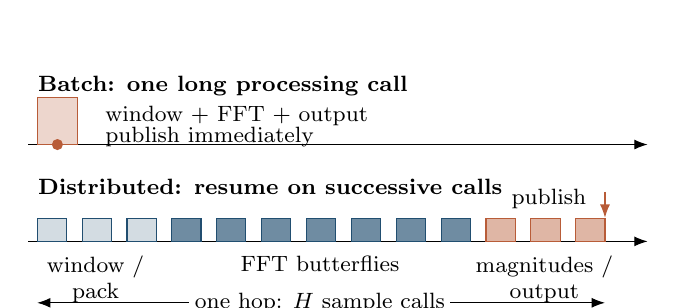
\begin{tikzpicture}[x=0.57cm,y=0.6cm,font=\footnotesize,>=Latex]
\node[anchor=west] at (0,3.1) {\textbf{Batch: one long processing call}};
\draw[->] (0,1.85) -- (13.8,1.85);
\draw[fill=accent!25,draw=accent] (0.2,1.85) rectangle (1.1,2.85);
\node[anchor=west] at (1.5,2.45) {window $+$ FFT $+$ output};
\fill[accent] (0.65,1.85) circle (2pt);
\node[anchor=west] at (1.5,2.02) {publish immediately};
\node[anchor=west] at (0,0.95) {\textbf{Distributed: resume on successive calls}};
\draw[->] (0,-0.2) -- (13.8,-0.2);
\foreach \x in {0.2,1.2,2.2} {
  \draw[fill=ink!20,draw=ink] (\x,-0.2) rectangle +(0.65,0.48);
}
\foreach \x in {3.2,4.2,5.2,6.2,7.2,8.2,9.2} {
  \draw[fill=ink!65,draw=ink] (\x,-0.2) rectangle +(0.65,0.48);
}
\foreach \x in {10.2,11.2,12.2} {
  \draw[fill=accent!45,draw=accent] (\x,-0.2) rectangle +(0.65,0.48);
}
\node[anchor=north,align=center] at (1.5,-0.3) {window /\\pack};
\node[anchor=north] at (6.5,-0.3) {FFT butterflies};
\node[anchor=north,align=center] at (11.5,-0.3) {magnitudes /\\output};
\draw[<->] (0.2,-1.5) -- (12.85,-1.5);
\node[fill=white,inner sep=2pt] at (6.5,-1.5) {one hop: $H$ sample calls};
\draw[->,accent] (12.85,0.85) -- (12.85,0.3);
\node[anchor=east] at (12.65,0.7) {publish};
\end{tikzpicture}
\caption{The same selected frame can be computed at its endpoint or spread
over the following hop. Input capture continues in both cases. Bars are
conceptual work slices, not timing measurements; stages and bar heights are
not to scale. The distributed result is published on the last call.}
\label{fig:schedule}
\end{figure}


\subsection{A resumable FFT}
An iterative radix-2 FFT traverses stages, groups within a stage, and pairs
within a group. A butterfly reads two coefficients, multiplies one by a
precomputed twiddle factor, and replaces the pair by their sum and difference.
Saving the current stage, group, and pair is enough to resume the traversal.
The coefficient array remains in place between calls. Pausing introduces no
new transform mathematics: when resumed, the next butterfly sees the same
operands that an uninterrupted traversal would have produced.

For real input, pair the windowed samples as
$z[m]=u_r[2m]+j u_r[2m+1]$ and compute an $M=N/2$ point complex FFT.
Standard real-spectrum reconstruction then produces the $K=M+1$ bins from
DC through Nyquist~\cite{sorensen1987}. The complex traversal contains
\begin{equation}
 B=\frac{M}{2}\log_2 M=\frac{N}{4}\log_2(N/2)
 \label{eq:butterflies}
\end{equation}
butterflies. The traversal indices require constant storage; the coefficient
and lookup arrays require $O(N)$ storage. Any partition of this ordered
traversal preserves the result within the same arithmetic implementation.
This does not imply bitwise agreement with a different FFT library.

\subsection{Include the work around the FFT}
The analyzer divides each frame into four stages
(Table~\ref{tab:stages}). First, it windows pairs of retained input samples
and stores them in the FFT's permuted order. Next, it executes the
butterflies. It then reconstructs positive-frequency bins and computes their
magnitudes. Finally, it applies enabled smoothing and emits display data one
bin at a time. Each stage finishes before the next begins; a sample call can
cross a stage boundary if it has work left to do.

\begin{table}[tb]
\centering\small
\begin{tabular}{@{}p{0.22\linewidth}p{0.55\linewidth}r@{}}
\toprule
Stage & One operation & Credits \\
\midrule
Prepare & Window, pack, and permute an input pair & $pM$ \\
Transform & Execute one complex butterfly & $B$ \\
Magnitude & Reconstruct one bin; compute magnitude and optional prefix sum & $K$ \\
Output & Smooth one bin and write its display data & $oK$ \\
\bottomrule
\end{tabular}
\caption{Scheduled stages for real input. $M=N/2$ pairs and $K=M+1$ bins
are processed in order. The last column gives the total credits per stage;
$p$ and $o$ are preparation and output weights.}
\label{tab:stages}
\end{table}


Frequency smoothing uses prefix sums of the magnitudes. Once those sums are
complete, the mean over any contiguous bin range needs two prefix reads and
a subtraction rather than a loop over that range. Temporal smoothing updates
one stored value per bin. Thus neither form of smoothing adds an unscheduled
whole-spectrum pass on the publication call. The display callback must also
perform bounded work per bin; an arbitrary expensive callback would defeat
the schedule.

To account for operations with different costs, the implementation assigns
integer \emph{credits}. Most operations use one credit. Rebuilding window
coefficients uses $p=4$ credits per input pair, compared with $p=1$ when the
cache is ready. Output uses $o=2$ credits per bin for Fourier's four-channel
display conversion and $o=1$ otherwise. A weighted operation executes at its
first credit; the remaining credits defer later work. These are engineering
weights, not measurements of equal execution time. The total is
\begin{equation}
 W=pM+B+(1+o)K.
 \label{eq:work}
\end{equation}
The weights affect where work falls within the hop without changing the
computed spectrum or the chosen publication time.

\subsection{An exact completion schedule}
Number a frame's sample calls $s=1,\ldots,H$, starting with the call that
captures its endpoint. Assign call $s$ the quota
\begin{equation}
 q_s=\floor{\frac{sW}{H}}-\floor{\frac{(s-1)W}{H}}.
 \label{eq:quota}
\end{equation}
The cumulative count after $s$ calls is $\floor{sW/H}$, so all $W$ credits
have been consumed after exactly $H$ calls. Every call receives either
$\floor{W/H}$ or $\ceil{W/H}$ credits. An integer quotient and remainder
implement the rule without dividing on every sample:
\begin{lstlisting}
// Once per frame configuration:
base = W / H; remainder = W % H;
// At frame start: error = 0.
// On each sample call:
quota = base;
error += remainder;
if (error >= H) { error -= H; ++quota; }
advance_analysis(quota);
if (++phase == H) { publish(); phase = 0; }
\end{lstlisting}
Here \code{advance\_analysis} consumes credits in the stage order above,
preserving the current stage and its cursor. Input capture occurs on every
call, including calls whose quota is zero. Publication waits for the fixed
boundary even if the last weighted operation has already executed.

For a clean scalar frame with $N=4096$ and $H=1024$, $W=17410$:
1022 calls consume 17 credits and two consume 18. For fixed configuration,
any 64 consecutive calls consume at most
$\ceil{64W/H}=1089$ credits, including blocks that cross a frame boundary.
More generally, when $H$ is proportional to $N$, the maximum per-sample
quota grows as $O(\log N)$ while a batch frame still requires
$O(N\log N)$ work at once. The schedule bounds operation counts, not
elapsed time: instruction costs, memory effects, and operating-system
interruptions are outside that arithmetic statement.

Keeping the frame clock separate from arithmetic completion is essential.
A fixed rounded quota such as $\ceil{B/H}$ butterflies per call can finish
early. Restarting immediately would change the actual update rate and any
smoothing calibrated to it. Equation~\eqref{eq:quota} distributes the
remainder across the intended interval and retains the requested cadence.

\subsection{Input lifetime and result delay}
The frame selected at $t_r$ is published at $t_r+H-1$. Measured from its
newest sample, the delay is therefore
\begin{equation}
 A_{\mathrm{endpoint}}=(H-1)/f_s.
 \label{eq:age}
\end{equation}
Measured from the window center, add $(N-1)/(2f_s)$. For the 4096-point,
1024-hop example at 48\,kHz, these ages are 21.31 and 63.97\,ms,
respectively. Even an immediate batch transform has the window-center age;
distribution adds the time spent advancing the frame. These are logical
sample-clock ages, excluding computation time, audio buffering, and repaint.

A preallocated input ring with capacity $N_{\max}+H_{\max}$ retains every
selected sample until analysis finishes. At most $H-1$ later samples arrive
before publication, so the oldest sample of the $N$-sample frame cannot be
overwritten. Windowing can therefore proceed incrementally without a bulk
frame copy. The first frames use zero padding for input that predates startup.
With fixed settings, only one frame is in progress and successive results are
published exactly $H$ samples apart.

\section{Implementation in VCV Rack}
\label{sec:implementation}
The method is implemented by the header-only C++ class
\code{SpectrumAnalysis<T>} and used by two modules in the Arhythmetic Units
plugin. Fourier displays four spectra, using the four lanes of Rack's SIMD
sample type as independent channels. Spectre displays a scalar spectrogram.
Neither module has an audio output, but both analyze input on the engine
thread. The scheduling code depends on arithmetic operations on \code{T},
not on Rack or its graphics API.

Storage and maximum-size twiddle and permutation tables are prepared before
sample processing. Smaller transforms reuse those tables by changing indices
and strides. Window coefficients are cached and rebuilt incrementally after
a relevant setting change. The scalar path retains the ordinary butterfly
traversal; dense SIMD work is dispatched in contiguous segments within the
same sample quota to reduce repeated setup. This preserves the scheduling
bound without requiring a function dispatch for every individual butterfly.

At each frame boundary the modules latch analysis settings. Length changes
invalidate input and averaging history logically; reset or sample-rate changes
cancel partial analysis. Smoothing and display-coordinate caches rebuild in
scheduled per-bin operations. Steady-state analysis and live window, length,
and smoothing changes use prepared storage. Increasing the sample rate can
require growing Fourier's input ring in the host's sample-rate callback;
that lifecycle operation is outside the per-sample guarantee.

Publishing a spectrum must not reintroduce a large copy or expose unfinished
data to the display. Each bin is written into producer-owned storage. At
completion, a single-producer/single-consumer mailbox exchanges ownership using
acquire/release atomics. The UI keeps its current slot while the engine fills
another. Fourier publishes a completed curve; Spectre publishes completed
history columns and constructs its image on the UI thread. A slow consumer
can miss intermediate updates, but it does not observe a partially written
spectrum. This ownership rule is separate from the arithmetic schedule.

The deployed defaults also make the latency choice concrete. Fourier uses
$N=2048$ and a 30\,ms hop ($H=1440$ at 48\,kHz); Spectre uses $N=2048$
and $H=1024$. Both default to a flattop window. The schedule adds nearly one
hop before publication, not one hop of audio output latency: these modules
produce display data only. Display polling and rendering add further delay.
The study below measures processing and logical publication age; it does not
evaluate the perceptual acceptability of that display response.

\section{Experimental Method}
\label{sec:evaluation}
The study asks three questions: how much of a burst reduction comes from work
placement within a fixed implementation; how that choice changes with native
kernels and completion horizon; and whether it improves complete-module
behavior under Rack's sample-synchronous engine. These questions and the
workload matrix were recorded before collection. The present analysis is a
\emph{descriptive pilot study}; it does not select and then confirm a winner.

\subsection{Host, sessions, and workload boundaries}
Two separately prepared sessions ran on September 30, 2026 (local time) on one
Apple M1 Pro laptop, with macOS 26.6.2 and Apple Clang 21.0.0. Both used the
same executable and archived sources. The operator declared networking and
Bluetooth disconnected and agents and unnecessary applications closed.
The runner required AC power and Low Power Mode off, held
\code{caffeinate -is} assertions, settled for 180 seconds after staging, and
settled each fresh process for one second before warmup. Pre/post snapshots
verify power and sleep assertions; they also show residual macOS service
activity, including \code{sandboxd} and Spotlight indexing. They cannot
establish the absence of interference during a particular interval.

Each session executed 194 planned cells twice in fresh processes, giving 776
processes in total. Three bridge cells repeat between groups: there are 191
unique full configurations. Group order was fixed; within-group process order
used the predeclared session seeds. We retain every process and slow interval.
Table~\ref{tab:study-design} describes the seven groups. Setup, plan creation,
correctness replay, storage probes, and output serialization are outside the
block timing intervals. These measurements replace the earlier manuscript's
performance campaign; old observations are retained only as historical artifacts.

\begin{table}[htbp]
\centering\small
\begin{tabular}{@{}lrll@{}}
\toprule
Group & Cells & Execution & Blocks/process \\
\midrule
Baselines & 24 & continuous & 4096 \\
Granularity & 39 & continuous & 960--4096 \\
Scaling & 16 & continuous & 1024--16384 \\
Modules & 9 & paced & 960--5760 \\
Stress & 12 & continuous & 1028--16384 \\
Host & 83 & paced & 1024--4096 \\
Lifecycle & 11 & continuous & 1024--16384 \\
\bottomrule
\end{tabular}
\caption{Predeclared pilot matrix: two sessions and two fresh processes per cell per session. Stream groups use 256 nominal hops, except Stress (128); host uses 262,144 engine samples. Lifecycle includes separate 65,536-sample event sequences and 1,048,576-sample decays. Each process has 16 warmup hops; host warmup rounds up to whole blocks. Three repeated bridge cells retain their group identities.}
\label{tab:study-design}
\end{table}


The stream harness measures complete analysis calls with a controlled sink,
or actual module \code{process()} paths including conditioning and display-data
conversion. Fourier's shipped defaults use four SIMD lanes, $N=2048$, a
30\,ms hop ($H=1440$ at 48\,kHz), and a flattop window. Spectre uses scalar
samples, $N=2048$, $H=1024$, and its flattop default. Controlled scalar
comparisons use a Hann window, $H=1024$, no smoothing, and $D=64$ unless
specified. All figures and tables state which boundary they compare.

The host group calls the pinned Rack engine's actual \code{stepBlock()},
including worker synchronization, with one or four engine threads, 0/1/4/16
analyzers, and 0/16/64 deterministic background modules. The host matrix is a
structured set of combinations, not a full factorial design. Native module
controls replace analysis inside the same module shell while retaining input
conditioning, display conversion, and mailbox publication. They retain some
unused production storage; their footprint is not an optimized replacement's
memory requirement. A concurrent headless consumer optionally copies and
checksums snapshots at 30 or 60\,Hz, with declared stalls. It does not draw a
window or drive an audio interface.

\subsection{Matched controls and native layouts}
The matched first-party batch and distributed controls use the same scalar
analysis implementation, arithmetic, and storage. They isolate placement more
closely than a comparison across FFT libraries. Native batch/hybrid pairs also
share the same retained-input, window, magnitude, smoothing, and output path.
Batch runs the sequence immediately; hybrid distributes its surrounding stages
but executes one indivisible native transform/reorder call. The native
pipeline uses contiguous ring segments and native output layouts, avoiding
per-element ring-modulo and canonical-complex conversion passes. vDSP uses
vector window/packing operations and batched four-channel transforms; FFTW
uses reusable real plans, including \code{plan\_many} for four channels;
PFFFT uses its ordered packed spectrum. Magnitudes use an explicitly scaled
norm to prevent avoidable squaring underflow. Thus these are stronger native
controls than the previous scalar-glue adapters, but not a claim to exhaust
every provider-specific optimization.

The granularity group holds frame hop fixed and changes native completion
horizon to $H_c\in\{H,\ceil{H/2},\ceil{H/4}\}$. Publication occurs at
endpoint age $H_c-1$, followed by idle capture until the next endpoint. This
changes latency and surrounding-stage density without subdividing the native
FFT. Native sub-FFT leaves and new stage weights were explicitly deferred;
neither has measured evidence in this study. Production weights $p=4$ for
window rebuild and $o=2$ for Fourier output were tuned in earlier engineering
experiments on this same M1 Pro. Band-cache rebuilding remains inside output
units without an additional weight. The new pilots are not independent
validation of those weight choices.

\subsection{Timing, replication, and age}
Continuous stream groups execute blocks back to back. The host group uses
absolute periodic releases at $D/f_s$, without resetting the release origin
after overruns. A monotonic clock records wake, start, and finish separately.
Inherited thread policy is used: no core affinity, frequency lock, or
real-time policy experiment is implied. Stream processes inherit and record
FPU control; the actual Rack engine applies Rack's block FPU policy. Empty
timer observations are retained without subtraction, and values are rounded
to approximately three significant figures.

The primary burst statistic is the median of \emph{per-hop peak block times}:
for each complete endpoint-to-next-endpoint interval, take the largest duration
of any whole block intersecting it. This includes a batch burst regardless of
its frequency among all callbacks. Shared blocks contribute to each intersected
hop; no sub-block costs are invented. Engine peaks use actual replay endpoints
and the full hop for both batch and delayed publication. Lifecycle sequences
are excluded from this stationary-hop statistic. Callback p99, maxima, and
counts above $D/f_s$ remain separate secondary observations.

Stream cost is the sum of instrumented block wall times divided by engine
samples. It includes timer/dispatch and interruption effects; this new design
contains no separate untimed-loop throughput pass. Host results additionally
retain process-wide user-plus-system CPU time across the measurement interval,
including workers, pacing overhead and any headless consumer. CPU and block
wall time are distinct quantities. A paced release miss means finish exceeds
the synthetic release deadline, including wake lateness and accumulated
backlog. A compute-budget exceedance means the timed block alone exceeds
$D/f_s$. Neither is an audio-device underrun.

For each cell we average the two process costs within each session; for burst
quantiles we take the median of the two process summaries. Tables show the
midpoint of the two session summaries, their range where indicated, and the
largest retained observation. There are only two session replicates, both on
the same date and host. Callbacks, hops, analyzers, and channels are dependent
observations. We report descriptive variation rather than confidence intervals,
rare-event probabilities or a worst-case execution-time claim
\cite{kalibera2013,mytkowicz2009,wilhelm2008}.

Publication age is measured in logical engine samples relative to the frame
endpoint; center age adds $(N-1)/2$. Consumer age is bounded by the completed
block watermarks observed around its copy, with one block of uncertainty.
Final drains are excluded from normal consumer ages. These sample-clock ages
are not wall-clock freshness during an overrun and do not include repaint.

\subsection{Numerical and provenance checks}
Every session passed checks of archive and artifact hashes, the exact declared
matrix and process order, execution sidecars, and all-output numerical replay.
Independent references use direct DFTs at small lengths and a separately
structured binary64 FFT at larger lengths; module replay also models DC
conditioning and display conversion. Ordinary magnitude-vector relative
$\ell_2$ and $\ell_\infty$ errors must be at most $3\times10^{-4}$ for float
or $10^{-10}$ for double; a zero reference requires zero output. These are
engineering acceptance budgets, not guarantees for each weak bin.

The long complete-module decay fixture separately flags the region affected
by Rack's flush-to-zero behavior and Fourier's display mapping. It uses the
predeclared \code{module-decay-ftz-v1} absolute floor, retains every vector,
and excludes flagged vectors from relative-accuracy claims. The floor is an
engineering allowance, not a proven error bound. This distinction matters:
relative error can reach one in that tail while the absolute error remains
below its recorded floor. Native allocator storage and allocation calls are
opaque to the separate C++ allocation probe. Appendix~\ref{app:reproducibility}
identifies the raw evidence and deterministic publication tools.

\section{Results}
\label{sec:results}
\subsection{Distribution reduces bursts, with overhead}
Table~\ref{tab:conference-baselines} isolates work placement and compares
native alternatives. Distributing the matched scalar implementation reduces
the typical hop peak from \StudyBatchPeak{} to
\StudyCorePeak\,$\mu$s, a factor of \StudyPlacementRatio. Aggregate
instrumented cost rises from \StudyBatchCost{} to
\StudyCoreCost\,ns/sample, an increase of about 18\%. The same FFT
arithmetic is being performed in smaller pieces; the result is less
concentrated execution rather than less total work.

\begin{table}[htbp]
\centering\small
\begin{tabular}{@{}lrr@{}}
\toprule
Analysis path & Cost & Peak [sessions] \\
\midrule
Matched batch & 68.3 & 52.2 [51.2--53.1] \\
Matched distributed & 80.3 & 6.67 [6.25--7.08] \\
PFFFT batch & 41.3 & 13.7 [13.1--14.3] \\
PFFFT hybrid & 49.8 & 8.15 [7.4--8.9] \\
vDSP batch & 43.6 & 17.1 [16.8--17.4] \\
vDSP hybrid & 59.4 & 8.92 [8.85--8.98] \\
FFTW batch & 41.3 & 21.8 [20.7--22.9] \\
FFTW hybrid & 46.6 & 12.5 [11.6--13.4] \\
\bottomrule
\end{tabular}
\caption{Scalar analysis, $N=4096$, $H=1024$, $D=64$, Hann, no smoothing. Cost is instrumented ns/sample; peak is the typical hop peak in $\mu$s. Brackets give the two session summaries. Each row contains four processes, 16,384 blocks, and 1,024 complete hops. No block exceeded the 1,333\,$\mu$s budget.}
\label{tab:conference-baselines}
\end{table}


All three native hybrids also lower the peak relative to their own batch
paths. PFFFT, for example, moves from \StudyPffftBatchPeak{} to
\StudyPffftHybridPeak\,$\mu$s while cost rises from
\StudyPffftBatchCost{} to \StudyPffftHybridCost\,ns/sample. Native hybrids
can therefore recover much of the burst reduction with lower aggregate cost
than the custom distributed transform. The fully distributed path has the
lowest typical peak at this scalar configuration, but it has the highest
cost. There is no single winner on both measures.

Across the campaign's three baseline lengths, four implementation families,
and two sessions, the distributed or hybrid member has the lower session
hop-peak summary in all 24 comparisons. These are related observations on one
machine, not 24 independent replications. Moreover, every typical peak in
Table~\ref{tab:conference-baselines} is small relative to the
1,333\,$\mu$s block budget. This experiment establishes the scheduling
effect; complete-host measurements determine whether the saved headroom is
substantial in a patch.

\subsection{A shorter schedule delivers earlier, larger bursts}
A native hybrid can finish within $H$, $H/2$, or $H/4$ sample calls, then
only capture input until the next frame endpoint. Table~\ref{tab:conference-horizons}
shows this tradeoff for four-channel vDSP analysis at a larger transform and
shorter hop. Reducing the completion interval from 240 to 60 calls cuts
endpoint-to-publication age from 4.98 to 1.23\,ms. The typical peak rises
from \StudyHorizonFullPeak{} to
\StudyHorizonQuarterPeak\,$\mu$s, approaching the batch peak of
125\,$\mu$s. The unchanged native transform remains indivisible; the
surrounding work becomes more densely packed.

\begin{table}[htbp]
\centering\small
\begin{tabular}{@{}lrrr@{}}
\toprule
Finish after & Age (ms) & Cost & Peak \\
\midrule
Batch & 0 & 544 & 125 \\
$H$ & 4.98 & 589 & 68.6 \\
$H/2$ & 2.48 & 594 & 95.4 \\
$H/4$ & 1.23 & 568 & 121 \\
\bottomrule
\end{tabular}
\caption{Four-channel vDSP analysis, $N=16384$, $H=240$, $D=64$, Hann. Age is endpoint-to-publication delay; cost is ns/sample for all four channels; peak is $\mu$s. Each row contains four processes and 3,840 blocks. Only the completion interval changes between hybrid rows.}
\label{tab:conference-horizons}
\end{table}


This configuration also shows a limit of the custom FFT. Its four-channel SIMD
path costs \StudySimdExtremeCost\,ns/sample with a
\StudySimdExtremePeak\,$\mu$s typical peak. The full-hop vDSP hybrid
costs \StudyHorizonFullCost\,ns/sample with a
\StudyHorizonFullPeak\,$\mu$s peak. Here the native hybrid is better on
both recorded measures. The benefit of interrupting every butterfly therefore
depends on transform size, hop, channel organization, and native kernel cost.

\subsection{The effect survives one host configuration}
With four aligned Fourier modules on one Rack engine thread, the distributed
implementation has a \StudyHostCorePeak\,$\mu$s typical hop peak,
compared with \StudyHostBatchPeak\,$\mu$s for native vDSP batch and
\StudyHostHybridPeak\,$\mu$s for the vDSP hybrid
(Table~\ref{tab:conference-host}). These occupy approximately 15\%, 67\%,
and 32\% of the block budget. Unlike the scalar comparison, the difference
is a substantial fraction of the time available to the rest of the patch.
The cost is higher aggregate processing: production uses
\StudyHostCoreCost\,ns/sample, versus \StudyHostBatchCost{} for batch and
\StudyHostHybridCost{} for hybrid. Both distributed paths also defer
publication by nearly the 30\,ms hop.

\begin{table}[htbp]
\centering\small
\begin{tabular}{@{}lrrr@{}}
\toprule
Analysis & Cost & Peak [sessions] & Misses \\
\midrule
Distributed & 2300 & 201 [197--206] & 18 \\
vDSP batch & 1730 & 890 [885--894] & 20 \\
vDSP hybrid & 2040 & 423 [417--428] & 38 \\
\bottomrule
\end{tabular}
\caption{Actual Rack engine: one thread, four aligned four-channel Fourier modules, $N=2048$, $H=1440$, $D=64$, flattop. Cost is block wall ns/sample for the complete engine; peak is $\mu$s. Brackets give session summaries. Misses are late synthetic releases across 16,384 blocks per row, including wake lateness, not audio underruns.}
\label{tab:conference-host}
\end{table}


With four engine threads and four aligned modules, the typical peaks converge
to about 100--115\,$\mu$s. Rack synchronizes its workers between
samples~\cite{rackengine}, but the experiment cannot isolate that cost from
core placement or power-state effects. The empty four-thread engine itself
consumes about three CPU-seconds per second of nominal audio, indicating that
its workers remain active between paced releases. The one-thread engine can
sleep. The contrast therefore changes more than available parallelism.

Alignment also matters. With sixteen modules on four threads, production's
typical peak is \StudyHostManyCorePeak\,$\mu$s, compared with
\StudyHostManyBatchPeak\,$\mu$s for aligned vDSP batch. Staggering the
batch modules lowers their peak to
\StudyHostStaggerBatchPeak\,$\mu$s. Phase distribution can reduce the
coincidence of complete transforms without making them resumable, although an
individual module cannot generally choose the phases of unrelated modules.

Lower typical peaks do not establish better deadline reliability. In the
one-thread, four-module comparison, production, vDSP batch, and hybrid miss
18, 20, and 38 synthetic releases respectively, across 16,384 blocks per row.
With sixteen aligned modules on four threads, production misses 19 releases
and vDSP batch misses none. Empty-engine controls also have late releases.
Wake delays, interruptions, and backlog remain relevant even when the normal
processing burst is much smaller than the deadline.

\subsection{Operating and numerical limits remain visible}
Direct paced calls to a default Fourier module have a typical peak of
\StudyModuleDefaultPeak\,$\mu$s. At $N=16384$ with a 5\,ms hop, the
four-port module reaches \StudyModuleExtremePeak\,$\mu$s; enabling both
smoothing modes raises this to \StudyModuleBothPeak\,$\mu$s and produces
196 compute-budget exceedances in 3,840 blocks. Scheduling distributes the
work but cannot make arbitrarily demanding settings affordable. No paced
native complete-module control was collected at this extreme configuration.

All numerical replays pass their declared acceptance policies. The largest
ordinary float relative vector errors are below $4.1\times10^{-5}$, against
a $3\times10^{-4}$ budget. These results include high overlap,
non-power-of-two hops, silence, and serialized lifecycle changes. Relative
error can reach one in the separately flagged long-decay tail; that region
is covered only by its absolute floor. The tests substantiate the implemented
analysis within those policies, not uniform relative accuracy for every weak
spectral component.

\section{Discussion and Limits}
\label{sec:discussion}
\subsection{When the tradeoff is useful}
The strongest case for cooperative analysis is a caller that values reducing
concentrated engine work and can tolerate an additional hop of spectrum age.
The representative comparison reduces callback p99 while increasing aggregate
cost. That is useful evidence for an engineering choice, not a new transform
complexity result. For a low-cost visualizer, headroom in the callback budget
may matter more than minimum arithmetic throughput; an application needing
fresh output or many concurrent analyzers may make the opposite choice.
The observed timing distributions cannot decide those application priorities.
For the representative $D=64$, 48\,kHz case, the nominal callback interval is
\PaperCmpBudgetUs\,$\mu$s: the production and vDSP p99 values occupy only
\PaperCmpCoreBudgetPercent\% and \PaperCmpVdspBudgetPercent\% of that interval,
respectively. Thus the measured reduction does not show that the native
baseline was near its deadline, or that redistribution prevented audible
failures. Such a claim would require a contended host and device measurements.

The PFFFT hybrid is a useful intermediate design: it distributes surrounding
work while keeping a native FFT indivisible. It shows that scheduling the
pipeline around a batch transform can capture some benefit without suspending
individual butterflies. Its comparison with the matched scheduled-batch
control isolates work placement more closely than a comparison with the
production analyzer, which also changes arithmetic, layout, storage, and
caching. The extra state in a resumable transform is justified only when its
measured behavior meets a requirement that the simpler alternative does not.

The inverse and chain results sharpen that qualification. Deferring butterfly
execution does not eliminate the bulk buffering and conjugation at job or
stage boundaries. The representative native PFFFT and vDSP inverse jobs provide both lower
aggregate cost and lower p99 than the incremental control. The complete-chain
control reduces p99 more modestly than its large aggregate-cost penalty. Thus the favorable
analysis example cannot be generalized to all frequency-domain processing.
The formulas in Section~\ref{sec:inverse-chain} identify what a future complete
inverse scheduler would need to change. The current measurements are already
useful as counterexamples to a blanket claim that incremental execution
reduces callbacks more effectively than optimized batch execution.

\subsection{Interpretation and external validity}
The primary tables compare declared input/output contracts. Smoothing
interval arithmetic and transform layouts differ across implementation
families; numerical agreement is within the stated contracts and budgets,
not bitwise identity. Precision, channel count, state, callback phase, and
additional DSP change the task. Extension results should be read within each
matched group rather than combined into a single provider score.

A high percentile, a maximum, and aggregate throughput answer different
questions. Single-sample p99 can omit frame work occurring less than once per
hundred calls. Maxima retain those bursts and rare preemptions but depend on
observation duration; the separate group durations preclude indiscriminate
maxima comparisons. No samples are trimmed and no empty-timer cost is
subtracted. Small absolute differences and sub-tick observations should not
be interpreted as finely resolved instruction costs. Storage probes measure
only their declared allocation scope; unknown provider-native storage prevents
a complete memory ranking.

All confirmation observations come from one compiler and one macOS ARM64 host
on one night. The prepared sessions expose temporal variation, including
unfavorable session excursions, but do not establish independent-host
replication or a stable rare-event distribution. Dynamic FFTW planning is part
of the recorded configuration. Other architectures, compilers, and plans may
change the relative costs. Binary64 references, deterministic fixtures, and
all-publication audits support the stated numerical workloads, not every
possible input or application-specific tolerance.

\subsection{Work bounds and real-time behavior}
The proof bounds credits in the complete analysis sequence. Unequal unit
costs, memory hierarchy, preemption, host lifecycle work, and unrelated DSP
still determine elapsed time. A late call executes its logical quota; the
scheduler does not recover a missed deadline. Producer publication also does
not guarantee display consumption or repaint cadence: a slow display may skip
complete snapshots by design.

The benchmark runs synchronously without an audio driver or concurrent UI.
It therefore provides no measured device underrun rate or proof of hard
real-time safety. Worker-thread analyzers, overlap-reusing sliding/hopping
methods, non-power-of-two transforms, and long-filter applications are not
ranked. Appendix~\ref{app:evaluation-agenda} identifies the next experiments.
The complete paper can support an implementation decision under its recorded
conditions; broader recommendations require those additional measurements.

\section{Conclusion}
Complete spectral analysis can be organized as bounded, dependency-ordered
operations with an exact publication hop. The resulting contract specifies
work-credit accounting, retained-input capacity, cancellation, and ownership
of completed spectra, while preserving the selected frame. Its scope extends
beyond suspending FFT butterflies to the surrounding preparation and output
stages that can otherwise concentrate work at frame boundaries.

That contract makes the performance question measurable; it does not answer
it by itself. Historical controls motivate the design, and the comparison
protocol separates changes in work placement from practical differences
between implementations. Final production evidence is needed to determine
where reductions in callback-duration tails justify additional total cost,
state, and spectrum age. No universal speedup or hard execution-time guarantee
follows from the scheduling bound.

\begin{thebibliography}{99}
\small\raggedright
\interlinepenalty=10000
\bibitem{rack}
VCV, ``Plugin API guide,'' \emph{VCV Rack Manual}. Accessed September 28, 2026.
\url{https://vcvrack.com/manual/PluginGuide}.
\bibitem{cooley1965}
J. W. Cooley and J. W. Tukey, ``An algorithm for the machine calculation of
complex Fourier series,'' \emph{Mathematics of Computation}, vol. 19, no. 90,
pp. 297--301, 1965. \href{https://doi.org/10.1090/S0025-5718-1965-0178586-1}{doi:10.1090/S0025-5718-1965-0178586-1}.

\bibitem{sorensen1987}
H. V. Sorensen, D. L. Jones, M. T. Heideman, and C. S. Burrus,
``Real-valued fast Fourier transform algorithms,'' \emph{IEEE Transactions
on Acoustics, Speech, and Signal Processing}, vol. 35, no. 6, pp. 849--863,
1987. \href{https://doi.org/10.1109/TASSP.1987.1165220}{doi:10.1109/TASSP.1987.1165220}.

\bibitem{allen1977}
J. B. Allen and L. R. Rabiner, ``A unified approach to short-time Fourier
analysis and synthesis,'' \emph{Proceedings of the IEEE}, vol. 65, no. 11,
pp. 1558--1564, 1977.
\href{https://doi.org/10.1109/PROC.1977.10770}{doi:10.1109/PROC.1977.10770}.

\bibitem{harris1978}
F. J. Harris, ``On the use of windows for harmonic analysis with the discrete
Fourier transform,'' \emph{Proceedings of the IEEE}, vol. 66, no. 1,
pp. 51--83, 1978.
\href{https://doi.org/10.1109/PROC.1978.10837}{doi:10.1109/PROC.1978.10837}.

\bibitem{lo1999}
P.-C. Lo and Y.-Y. Lee, ``Real-time FFT algorithm applied to on-line spectral
analysis,'' \emph{Circuits, Systems, and Signal Processing}, vol. 18, no. 4,
pp. 377--393, 1999.
\href{https://doi.org/10.1007/BF01200789}{doi:10.1007/BF01200789}.

\bibitem{hurchalla2010}
J. Hurchalla, ``A time distributed FFT for efficient low latency convolution,''
in \emph{129th Audio Engineering Society Convention}, paper 8257, 2010.
\url{https://secure.aes.org/forum/pubs/conventions/?elib=15679}.

\bibitem{battenberg2011}
E. Battenberg and R. Avi\v{z}ienis, ``Implementing real-time partitioned
convolution algorithms on conventional operating systems,'' in
\emph{Proceedings of the 14th International Conference on Digital Audio
Effects (DAFx-11)}, Paris, France, September 2011.
\url{https://ericbattenberg.com/pdf/partconvDAFx2011.pdf}.

\bibitem{jacobsen2003}
E. Jacobsen and R. Lyons, ``The sliding DFT,'' \emph{IEEE Signal Processing
Magazine}, vol. 20, no. 2, pp. 74--80, 2003.
\href{https://doi.org/10.1109/MSP.2003.1184347}{doi:10.1109/MSP.2003.1184347}.

\bibitem{frigo2005}
M. Frigo and S. G. Johnson, ``The design and implementation of FFTW3,''
\emph{Proceedings of the IEEE}, vol. 93, no. 2, pp. 216--231, 2005.
\href{https://doi.org/10.1109/JPROC.2004.840301}{doi:10.1109/JPROC.2004.840301}.
Planner API: \url{https://www.fftw.org/fftw3_doc/Planner-Flags.html}
(accessed September 30, 2026).

\bibitem{pffft}
J. Pommier and contributors, ``PFFFT: A pretty fast FFT,'' software;
VCV Rack integration, \code{dsp::RealFFT}. Accessed September 30, 2026.
\url{https://github.com/VCVRack/pffft}.
\href{https://github.com/VCVRack/Rack/blob/v2/include/dsp/fft.hpp}{Rack FFT wrapper source}.

\bibitem{vdsp}
Apple, ``Using Fourier Transforms,''
\href{https://developer.apple.com/library/archive/documentation/Performance/Conceptual/vDSP_Programming_Guide/UsingFourierTransforms/UsingFourierTransforms.html}{\emph{vDSP Programming Guide}},
Accelerate framework documentation. Accessed September 30, 2026.

\bibitem{kalibera2013}
T. Kalibera and R. Jones, ``Rigorous benchmarking in reasonable time,'' in
\emph{Proceedings of the 2013 International Symposium on Memory Management
(ISMM '13)}, pp. 63--74, 2013.
\href{https://doi.org/10.1145/2464157.2464160}{doi:10.1145/2464157.2464160}.
Corrected author manuscript: \url{https://kar.kent.ac.uk/33611/}.

\bibitem{rackengine}
VCV, ``Rack engine implementation,'' source revision
\code{8c33d966d329e4a6e354593b2b5f9ac2df5a03bd}, inspected September 30, 2026.
\url{https://github.com/VCVRack/Rack/blob/8c33d966d329e4a6e354593b2b5f9ac2df5a03bd/src/engine/Engine.cpp}.

\end{thebibliography}

\end{document}
